%% LyX 2.3.6 created this file.  For more info, see http://www.lyx.org/.
%% Do not edit unless you really know what you are doing.
\documentclass[journal,article,submit,pdftex,moreauthors]{mdpi}
\usepackage[utf8]{inputenc}
\usepackage{float}
\usepackage{url}
\usepackage{amsmath}
\usepackage{graphicx}

\makeatletter

%%%%%%%%%%%%%%%%%%%%%%%%%%%%%% LyX specific LaTeX commands.

\Title{Locate the parameters of RBF networks using a hybrid Particle Swarm
Optimization method}

\TitleCitation{Locate the parameters of RBF networks using a hybrid Particle Swarm
Optimization method}

\newcommand{\orcidauthorA}{0000-0000-0000-000X}


\newcommand{\orcidauthorB}{0000-0000-0000-000X}


\Author{Ioannis G. Tsoulos$^{1,\dagger,\ddagger,*}$\orcidA{}, Vasileios
Charilogis$^{2,\dagger}$\orcidB{} $^{2,}$}

\AuthorNames{Ioannis G. Tsoulos, Vasileios Charilogis }

\AuthorCitation{Tsoulos, I.G.; Charilogis V.}


\address{$^{1}$\quad{}Department of Informatics and Telecommunications,
University of Ioannina, Greece; itsoulos@uoi.gr\\
$^{2}$\quad{}Department of Informatics and Telecommunications, University
of Ioannina, Greece; v.charilog@uoi.gr}


\corres{Correspondence: itsoulos@uoi.gr;}


\firstnote{Current address: Department of Informatics and Telecommunications,
University of Ioannina, Greece.}


\secondnote{These authors contributed equally to this work.}


\abstract{In the present work, an innovative two-phase method is presented
for parameter tuning in Radial Basis Function artificial neural networks.
These kinds of machine learning models find application in many scientific
fields in classification problems or in function regression. In the
first phase, a technique based on Particle Swarm Optimization is performed
to find a promising interval of values for the network parameters.
Particle swarm optimization was used as it is a highly reliable method
for global optimization problems and, in addition, it is one of the
fastest and most flexible techniques of its class. In the second phase,
the network is trained within the optimal interval using a global
optimization technique such as a Genetic Algorithm. Furthermore, in
order to speed up the training of the network and due to the use of
a two-stage method, parallel programming techniques were utilized.
The new method was applied to a number of well-known classification
and regression datasets, and the results were more than promising.}


\keyword{Neural networks; Particle Swarm Optimization; Genetic algorithms}

\DeclareTextSymbolDefault{\textquotedbl}{T1}
%% Because html converters don't know tabularnewline
\providecommand{\tabularnewline}{\\}
\floatstyle{ruled}
\newfloat{algorithm}{tbp}{loa}
\providecommand{\algorithmname}{Algorithm}
\floatname{algorithm}{\protect\algorithmname}

%%%%%%%%%%%%%%%%%%%%%%%%%%%%%% User specified LaTeX commands.
%  LaTeX support: latex@mdpi.com 
%  For support, please attach all files needed for compiling as well as the log file, and specify your operating system, LaTeX version, and LaTeX editor.

%=================================================================


% For posting an early version of this manuscript as a preprint, you may use "preprints" as the journal and change "submit" to "accept". The document class line would be, e.g., \documentclass[preprints,article,accept,moreauthors,pdftex]{mdpi}. This is especially recommended for submission to arXiv, where line numbers should be removed before posting. For preprints.org, the editorial staff will make this change immediately prior to posting.

%--------------------
% Class Options:
%--------------------
%----------
% journal
%----------
% Choose between the following MDPI journals:
% acoustics, actuators, addictions, admsci, adolescents, aerospace, agriculture, agriengineering, agronomy, ai, algorithms, allergies, alloys, analytica, animals, antibiotics, antibodies, antioxidants, applbiosci, appliedchem, appliedmath, applmech, applmicrobiol, applnano, applsci, aquacj, architecture, arts, asc, asi, astronomy, atmosphere, atoms, audiolres, automation, axioms, bacteria, batteries, bdcc, behavsci, beverages, biochem, bioengineering, biologics, biology, biomass, biomechanics, biomed, biomedicines, biomedinformatics, biomimetics, biomolecules, biophysica, biosensors, biotech, birds, bloods, blsf, brainsci, breath, buildings, businesses, cancers, carbon, cardiogenetics, catalysts, cells, ceramics, challenges, chemengineering, chemistry, chemosensors, chemproc, children, chips, cimb, civileng, cleantechnol, climate, clinpract, clockssleep, cmd, coasts, coatings, colloids, colorants, commodities, compounds, computation, computers, condensedmatter, conservation, constrmater, cosmetics, covid, crops, cryptography, crystals, csmf, ctn, curroncol, currophthalmol, cyber, dairy, data, dentistry, dermato, dermatopathology, designs, diabetology, diagnostics, dietetics, digital, disabilities, diseases, diversity, dna, drones, dynamics, earth, ebj, ecologies, econometrics, economies, education, ejihpe, electricity, electrochem, electronicmat, electronics, encyclopedia, endocrines, energies, eng, engproc, ent, entomology, entropy, environments, environsciproc, epidemiologia, epigenomes, est, fermentation, fibers, fintech, fire, fishes, fluids, foods, forecasting, forensicsci, forests, foundations, fractalfract, fuels, futureinternet, futureparasites, futurepharmacol, futurephys, futuretransp, galaxies, games, gases, gastroent, gastrointestdisord, gels, genealogy, genes, geographies, geohazards, geomatics, geosciences, geotechnics, geriatrics, hazardousmatters, healthcare, hearts, hemato, heritage, highthroughput, histories, horticulturae, humanities, humans, hydrobiology, hydrogen, hydrology, hygiene, idr, ijerph, ijfs, ijgi, ijms, ijns, ijtm, ijtpp, immuno, informatics, information, infrastructures, inorganics, insects, instruments, inventions, iot, j, jal, jcdd, jcm, jcp, jcs, jdb, jeta, jfb, jfmk, jimaging, jintelligence, jlpea, jmmp, jmp, jmse, jne, jnt, jof, joitmc, jor, journalmedia, jox, jpm, jrfm, jsan, jtaer, jzbg, kidney, kidneydial, knowledge, land, languages, laws, life, liquids, literature, livers, logics, logistics, lubricants, lymphatics, machines, macromol, magnetism, magnetochemistry, make, marinedrugs, materials, materproc, mathematics, mca, measurements, medicina, medicines, medsci, membranes, merits, metabolites, metals, meteorology, methane, metrology, micro, microarrays, microbiolres, micromachines, microorganisms, microplastics, minerals, mining, modelling, molbank, molecules, mps, msf, mti, muscles, nanoenergyadv, nanomanufacturing, nanomaterials, ncrna, network, neuroglia, neurolint, neurosci, nitrogen, notspecified, nri, nursrep, nutraceuticals, nutrients, obesities, oceans, ohbm, onco, oncopathology, optics, oral, organics, organoids, osteology, oxygen, parasites, parasitologia, particles, pathogens, pathophysiology, pediatrrep, pharmaceuticals, pharmaceutics, pharmacoepidemiology, pharmacy, philosophies, photochem, photonics, phycology, physchem, physics, physiologia, plants, plasma, pollutants, polymers, polysaccharides, poultry, powders, preprints, proceedings, processes, prosthesis, proteomes, psf, psych, psychiatryint, psychoactives, publications, quantumrep, quaternary, qubs, radiation, reactions, recycling, regeneration, religions, remotesensing, reports, reprodmed, resources, rheumato, risks, robotics, ruminants, safety, sci, scipharm, seeds, sensors, separations, sexes, signals, sinusitis, skins, smartcities, sna, societies, socsci, software, soilsystems, solar, solids, sports, standards, stats, stresses, surfaces, surgeries, suschem, sustainability, symmetry, synbio, systems, taxonomy, technologies, telecom, test, textiles, thalassrep, thermo, tomography, tourismhosp, toxics, toxins, transplantology, transportation, traumacare, traumas, tropicalmed, universe, urbansci, uro, vaccines, vehicles, venereology, vetsci, vibration, viruses, vision, waste, water, wem, wevj, wind, women, world, youth, zoonoticdis 

%---------
% article
%---------
% The default type of manuscript is "article", but can be replaced by: 
% abstract, addendum, article, book, bookreview, briefreport, casereport, comment, commentary, communication, conferenceproceedings, correction, conferencereport, entry, expressionofconcern, extendedabstract, datadescriptor, editorial, essay, erratum, hypothesis, interestingimage, obituary, opinion, projectreport, reply, retraction, review, perspective, protocol, shortnote, studyprotocol, systematicreview, supfile, technicalnote, viewpoint, guidelines, registeredreport, tutorial
% supfile = supplementary materials

%----------
% submit
%----------
% The class option "submit" will be changed to "accept" by the Editorial Office when the paper is accepted. This will only make changes to the frontpage (e.g., the logo of the journal will get visible), the headings, and the copyright information. Also, line numbering will be removed. Journal info and pagination for accepted papers will also be assigned by the Editorial Office.

%------------------
% moreauthors
%------------------
% If there is only one author the class option oneauthor should be used. Otherwise use the class option moreauthors.

%---------
% pdftex
%---------
% The option pdftex is for use with pdfLaTeX. If eps figures are used, remove the option pdftex and use LaTeX and dvi2pdf.

%=================================================================
% MDPI internal commands
\firstpage{1} 
 
\setcounter{page}{\@firstpage} 

\pubvolume{1}
\issuenum{1}
\articlenumber{0}
\pubyear{2022}
\copyrightyear{2022}
%\externaleditor{Academic Editor: Firstname Lastname} % For journal Automation, please change Academic Editor to "Communicated by"
\datereceived{} 
\dateaccepted{} 
\datepublished{} 
%\datecorrected{} % Corrected papers include a "Corrected: XXX" date in the original paper.
%\dateretracted{} % Corrected papers include a "Retracted: XXX" date in the original paper.
\hreflink{https://doi.org/} % If needed use \linebreak
%\doinum{}
%------------------------------------------------------------------
% The following line should be uncommented if the LaTeX file is uploaded to arXiv.org
%\pdfoutput=1

%=================================================================
% Add packages and commands here. The following packages are loaded in our class file: fontenc, inputenc, calc, indentfirst, fancyhdr, graphicx, epstopdf, lastpage, ifthen, lineno, float, amsmath, setspace, enumitem, mathpazo, booktabs, titlesec, etoolbox, tabto, xcolor, soul, multirow, microtype, tikz, totcount, changepage, attrib, upgreek, cleveref, amsthm, hyphenat, natbib, hyperref, footmisc, url, geometry, newfloat, caption

%=================================================================
%% Please use the following mathematics environments: Theorem, Lemma, Corollary, Proposition, Characterization, Property, Problem, Example, ExamplesandDefinitions, Hypothesis, Remark, Definition, Notation, Assumption
%% For proofs, please use the proof environment (the amsthm package is loaded by the MDPI class).

%=================================================================
% The fields PACS, MSC, and JEL may be left empty or commented out if not applicable
%\PACS{J0101}
%\MSC{}
%\JEL{}

%%%%%%%%%%%%%%%%%%%%%%%%%%%%%%%%%%%%%%%%%%
% Only for the journal Diversity
%\LSID{\url{http://}}

%%%%%%%%%%%%%%%%%%%%%%%%%%%%%%%%%%%%%%%%%%
% Only for the journal Applied Sciences:
%\featuredapplication{Authors are encouraged to provide a concise description of the specific application or a potential application of the work. This section is not mandatory.}
%%%%%%%%%%%%%%%%%%%%%%%%%%%%%%%%%%%%%%%%%%

%%%%%%%%%%%%%%%%%%%%%%%%%%%%%%%%%%%%%%%%%%
% Only for the journal Data:
%\dataset{DOI number or link to the deposited data set in cases where the data set is published or set to be published separately. If the data set is submitted and will be published as a supplement to this paper in the journal Data, this field will be filled by the editors of the journal. In this case, please make sure to submit the data set as a supplement when entering your manuscript into our manuscript editorial system.}

%\datasetlicense{license under which the data set is made available (CC0, CC-BY, CC-BY-SA, CC-BY-NC, etc.)}

%%%%%%%%%%%%%%%%%%%%%%%%%%%%%%%%%%%%%%%%%%
% Only for the journal Toxins
%\keycontribution{The breakthroughs or highlights of the manuscript. Authors can write one or two sentences to describe the most important part of the paper.}

%%%%%%%%%%%%%%%%%%%%%%%%%%%%%%%%%%%%%%%%%%
% Only for the journal Encyclopedia
%\encyclopediadef{Instead of the abstract}
%\entrylink{The Link to this entry published on the encyclopedia platform.}
%%%%%%%%%%%%%%%%%%%%%%%%%%%%%%%%%%%%%%%%%%

\makeatother

\begin{document}
\maketitle

\section{Introduction}

Regression and data classification are two major categories of problems
that are solved with machine learning techniques. Such problems appear
regularly in scientific areas such as physics \citep{physics_ml1,physics_ml2},
chemistry \citep{chemistry_ml1,chemistry_ml2}, economics \citep{econ_ml1,econ_ml2},
medicine \citep{med_ml1,med_ml2}, etc. A programming tool that is
used quite often to handle such problems is the Radial Basis Function
(RBF) artificial neural network \citep{rbf1}. An RBF network can
be expressed as a function:\textbf{
\begin{equation}
y\left(\overrightarrow{x}\right)=\sum_{i=1}^{k}w_{i}\phi\left(\left\Vert \overrightarrow{x}-\overrightarrow{c_{i}}\right\Vert \right)\label{eq:firstrbf}
\end{equation}
}The following applies to the above equation
\begin{enumerate}
\item The vector $\overrightarrow{x}$ is the input pattern to the equation.
The number of values in this vector is denoted as $d$.
\item The vectors $\overrightarrow{c_{i}},\ i=1,..,k$ are denoted as the
center vectors.
\item The vector $\overrightarrow{w}$ is considered as the output weight
of the RBF network.
\item The value $y\left(\overrightarrow{x}\right)$ is the predicted value
of the network for the pattern $\overrightarrow{x}$.
\end{enumerate}
Typically, the Gaussian function can bed used as the function $\phi(x)$
and it defined as:\textbf{
\begin{equation}
\phi(x)=\exp\left(-\frac{\left(x-c\right)^{2}}{\sigma^{2}}\right)
\end{equation}
}A plot for the Gaussian function with $c=0,\ \sigma=1$ is displayed
in Figure \ref{fig:gauss}. As it is observed, the value of the function
decreases as we move away from the center. An extensive overview of
RBF networks is given in the work of Ghosh and Nag \citep{rbfghosh}.
RBF networks are used as approximation tools in various cases, such
as  solutions of differential equations \citep{rbfde1,rbfde2},\textbf{
}digital communications \citep{rbfnetwork1,rbfnetwork2},\textbf{
}physics \citep{rbfphysics1,rbfphysics2}, chemistry \citep{rbfchemistry1,rbfchemistry2},\textbf{
}economics \citep{rbfecon0,rbfecon1,rbfecon2}, network security \citep{rbf_dos1,rbf_dos2}
etc. RBF networks are thoroughly discussed in\textbf{ }\citep{rbfadv}
and it has been parallelized in a variety of research papers \citep{rbfpar1,rbfpar2}.
This model has been extended by various researchers in tasks such
as creating new initialization techniques for the network parameters,\textbf{
}\citep{rbfinit1,rbfinit2,rbfinit3}, pruning techniques\textbf{ }\citep{rbfprun1,rbfprun2,rbfprun3},
construction of RBF networks \citep{rbfcon1,rbfcon2,rbfcon3} etc. 

In the current work, a hybrid technique is proposed for the optimal
calculation of the parameters of an RBF network. This technique consists
of two phases. During the first phase, information is collected from
the training data of the neural network and an attempt is made to
identify a small interval of values for the neural network parameters.
To identify this interval, an optimization method is used, which gradually
creates the optimal value interval, which is estimated to give the
lowest value for the training error of the network. To locate the
optimal interval, the particle swarm optimization (PSO) technique
is used \citep{psoTutorial}. The PSO method was chosen for the first
phase because it is fast and flexible enough for optimization problems,
does not require a large number of parameters to be input by the user,
and has been successfully used in a variety of problems such as flow
shop scheduling \citep{psoApp1}, developing charging strategies for
electric vehicles \citep{psoApp2}, emotion recognition \citep{psoApp3},
robot trajectory planning \citep{psoApp4} etc. The detection of the
value interval is performed in order to then make the minimization
of the network error faster and more efficient in the second phase
optimization method. In the second phase, the parameters of the neural
network are optimized within the optimal value interval of the first
phase. The optimization can be performed by any global optimization
method \citep{goReview}. In this work, the genetic algorithms \citep{ga1,ga2,ga3}
were chosen for the second phase. The main advantages of genetic algorithms
are tolerance on errors, easy to implement in parallel, efficient
exploration of the search space etc. 

Recently, many work has been appeared to tune the parameters of machine
learning models, such as the work of Agarwal and Bhanot \citep{rbftune}
for the adaptation of the RBF parameters, the incorporation of an
improved ABC algorithm to adapt the parameters of RBF networks \citep{rbfABC},
the usage of the Firefly algorithm for optimization \citep{fireflyMain}
along with machine learning models for Cervical cancer diagnosis \citep{fireflyCancer},
adaptation of CNN and XGBOOST models by an optimization algorithm
for COVID-19 diagnosis \citep{hybridCNN} etc.

The rest of this article is organized as follows: in section \ref{sec:Method-description}
the two phases of the proposed method are thoroughly discussed, in
section \ref{sec:Experiments} the experimental datasets are listed
as well as the experimental results and finally in section \ref{sec:Conclusions}
some conclusions are presented.

\begin{figure}[H]
\centering{}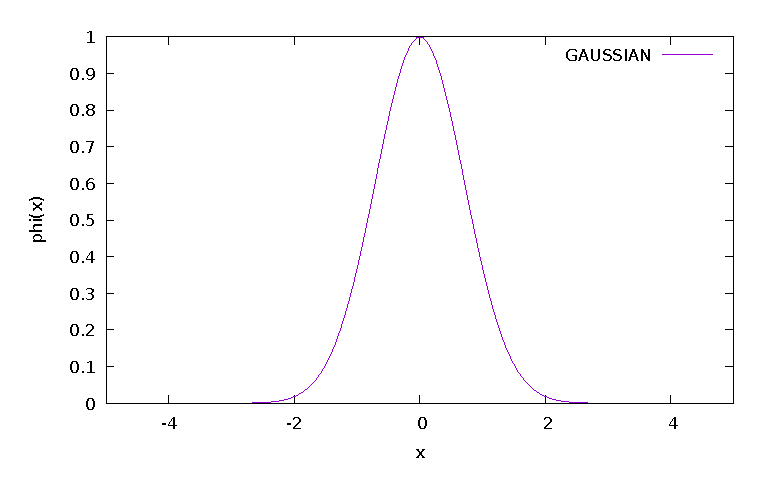
\includegraphics{gaussian}\caption{A typical plot for the Gaussian function, for $c=0$ and $\sigma=1$.\label{fig:gauss}}
\end{figure}


\section{Method description\label{sec:Method-description}}

The training error of the RBF network is expressed as: 
\begin{equation}
E(y(x,g))=\sum_{i=1}^{m}\left(y\left(x_{i},g\right)-t_{i}\right)^{2}\label{eq:eqrbf}
\end{equation}
The value $m$ stands for the number of patterns and $t_{i}$ is the
actual output for pattern $x_{i}$. The vector $g$ is the set of
the parameters of the RBF network. Usually, RBF networks are trained
through a two-phase procedure: 
\begin{enumerate}
\item In the first phase the $k$ centers as well as the associated variances
are estimated through K-Means algorithm \citep{kmeans}. A typical
formulation of the K-Means algorithm is outlined in Algorithm \ref{alg:The-K-Means-algorithm.}.
\item In the second phase, the weight vector $\overrightarrow{w}=\left(w_{1},w_{2},\ldots,w_{k}\right)$
is estimated by solving a linear system of equations.
\begin{enumerate}
\item \textbf{Set} \textbf{$W=w_{kj}$}
\item \textbf{Set} \textbf{$\Phi=\phi_{j}\left(x_{i}\right)$}
\item \textbf{Set $T=\left\{ t_{i}=f\left(x_{i}\right),i=1,..,M\right\} $. }
\item The system to be solved is identified as:\textbf{ 
\begin{equation}
\Phi^{T}\left(T-\Phi W^{T}\right)=0
\end{equation}
}With solution:\textbf{
\begin{equation}
W^{T}=\left(\Phi^{T}\Phi\right)^{-1}\Phi^{T}T=\Phi^{\dagger}T\label{eq:eqoutput}
\end{equation}
}
\end{enumerate}
\end{enumerate}
The proposed work uses two computational phases to optimally calculate
the network parameters. In the first phase, a promising range for
the parameters of the network is calculated through an optimization
process that incorporates interval arithmetic. In the second phase,
the parameters of the network are trained with the usage of a genetic
algorithm inside the located range of the first phase. The following
subsections analyze both of these phases in detail.

\begin{algorithm}
\caption{The K-Means algorithm.\label{alg:The-K-Means-algorithm.}}

\begin{enumerate}
\item \textbf{Repeat}
\begin{enumerate}
\item $S_{j}=\left\{ \right\} ,\ j=1..k$
\item \textbf{For} each sample $x_{i},\ i=1,...,m$ \textbf{do}
\begin{enumerate}
\item \textbf{Calculate} $j^{*}=\min_{i=1}^{k}\left\{ D\left(x_{i},c_{j}\right)\right\} $.
\item \textbf{Update} $S_{j^{*}}=S_{j^{*}}\cup\left\{ x_{i}\right\} $.
\end{enumerate}
\item \textbf{EndFor}
\item \textbf{For} each center $c_{j},\ j=1..k$ \textbf{do}
\begin{enumerate}
\item \textbf{Define} $M_{j}$ as the number of points in $S_{j}$
\item \textbf{Calculate }$c_{j}$
\[
c_{j}=\frac{1}{M_{j}}\sum_{i=1}^{M_{j}}x_{i}
\]
\end{enumerate}
\item \textbf{EndFor}
\end{enumerate}
\item \textbf{Calculate} the variances for every center as 
\[
\sigma_{j}^{2}=\frac{\sum_{i=1}^{M_{j}}\left(x_{i}-c_{j}\right)^{2}}{M_{j}}
\]
\item \textbf{Terminate }if there is no change in centers $c_{j}$.
\end{enumerate}
\end{algorithm}


\subsection{Preliminaries }

In order to perform interval arithmetic on RBF networks the following
definitions are introduced:
\begin{enumerate}
\item The comparison of two intervals $W=\left[w_{1},w_{2}\right]$, $Z=\left[z_{1},z_{2}\right]$
is performed through the function 
\begin{eqnarray}
L^{*}(W,Z) & = & \begin{cases}
\mbox{TRUE}, & w_{1}<z_{1},\mbox{OR\ \ensuremath{\left(w_{1}=z_{1}\ \mbox{AND}\ w_{2}<z_{2}\right)}}\\
\mbox{FALSE}, & \mbox{\mbox{OTHERWISE}}
\end{cases}\label{eq:eql}
\end{eqnarray}
\item The function $E(y)$ (equation \ref{eq:eqrbf}) is modified to an
interval one $\left[E_{\mbox{min}}(y),E_{\mbox{max}}(y)\right]$ calculated
with the procedure given in Algorithm \ref{alg:Fitness-calculation-for}.
\end{enumerate}
In the proposed algorithm, the RBF network contains $n$ variables,
where
\begin{equation}
n=(d+2)\times k
\end{equation}
 The value of $n$ is calculated as follows:
\begin{enumerate}
\item Every center $\overrightarrow{c_{i}},\ i=1,..,k$ has $d$ variables,
which means $d\times k$ variables.
\item For every center, a separate value $\sigma_{i}$ is used for the Gaussian
processing unit, which means $k$ variables.
\item The output weight $\overrightarrow{w}$ also has $k$ variables.
\end{enumerate}

\subsection{The proposed PSO algorithm\label{subsec:The-proposed-PSO}}

During this phase, arithmetic interval techniques are used to find
a suitable range for the parameters of the RBF network. The interval
techniques \citep{interval0,interval1,interval2} are a common method
in global optimization with various applications \citep{interval_app1,interval_app2,interval_app3}.
The first phase aims to locate the most promising bounding box for
the $n$ parameters of the corresponding neural network. The initial
bounding box is defined as\textbf{ $S$ }which is a subset of $\mathbb{R^{\mbox{n}}}$:\textbf{
\begin{equation}
S=\left[a_{1},b_{1}\right]\otimes\left[a_{2},b_{2}\right]\otimes\ldots\left[a_{n},b_{n}\right]\label{eq:eq2}
\end{equation}
}The interval method of the first phase divides the set $S$ subsequently
by discarding areas that are not promising enough to contain the global
minimum. In order to locate the best interval for the parameters of
the network, a modified PSO algorithm \citep{pso1} is used. The proposed
variant of the PSO method is based on the original technique (algorithm
1 of\citep{pso1} ) but the particles are intervals of values and
at each iteration a normalization of the velocity vector takes place
to avoid generating particles outside the original range of values.\textbf{
}The PSO method is a global optimization method based on a population
of candidate solutions, which in most cases are called particles.
The method is based on two vectors: the current location of particles
denoted as $\overrightarrow{p}$ and the velocity of their movement
denoted as $\overrightarrow{u}$. The PSO method finds the global
minimum by moving the particles based on their previous best position
as well as the best position of the total population of particles. 

The initial bounding boxes for the centers and variances of the RBF
network are constructed using the K-Means clustering algorithm. Subsequently,
the initial values for the intervals $\left[a_{i},b_{i}\right]$ are
calculated through the algorithm \ref{alg:initialValues}. The values
for the intervals of the first $(d+1)\times k$ variables are obtained
as a multiple of the positive quantity $F$ with the values obtained
by the K-Means. The value $B$ is used to initialize the intervals
for the output weight $\overrightarrow{w}$. Afterwards, the following
PSO variant is executed:
\begin{enumerate}
\item \textbf{Set} $N_{c}$ the number of particles.
\item \textbf{Set} the normalization factor $\lambda$.
\item \textbf{Set} the $k$ weights of the RBF network.
\item \textbf{Set} $N_{g}$ the maximum number of generations allowed.
\item \textbf{Set} $N_{s}$ the number of random samples that will be used
in the fitness calculation algorithm.
\item \textbf{Set} $f^{*}=\left[\infty,\infty\right]$, the fitness of the
best located particle $p^{*}$.
\item \textbf{Construct} $S=\left[a_{1},b_{1}\right]\otimes\left[a_{2},b_{2}\right]\otimes\ldots\left[a_{n},b_{n}\right]$,
as obtained from the previous two algorithms.
\item \textbf{Initialize} the $N_{g}$ particles. Each particle $p_{i},\ i=1,...,N_{c}$
is considered as a set of intervals randomly initialized in $S$.
The layout of each particle is graphically presented in Figure \ref{fig:The-layout-of}.
\item \textbf{For} $i=1,...,N_{c}$ \textbf{do }
\begin{enumerate}
\item \textbf{Calculate} the fitness $f_{i}$ of particle $p_{i}$ using
the procedure outlined in Algorithm \ref{alg:Fitness-calculation-for}.
\item \textbf{If} $L^{*}\left(f_{i},f^{*}\right)=\mbox{TRUE}$ \textbf{then}
$f^{*}=f_{i},\ p^{*}=p_{i}$
\item \textbf{Set} $p_{b,i}=p_{i},\ f_{b,i}=f_{i}$ the best located position
for particle $i$ and the associated fitness value.
\item \textbf{For} $j=1,...,n$ \textbf{do}
\begin{enumerate}
\item \textbf{Set} $\delta$ the width of interval $p_{ij}$
\item \textbf{Set} $u_{ij}=\left[-r\frac{\delta}{20},r\frac{\delta}{20}\right]$,
with $r$ being a random number in $[0,1]$. The velocity is initialized
to a small sub-interval of the range of values for the corresponding
parameter in order to avoid, as far as possible, excessive values
for the velocity. This would result in the particles moving out of
their value range very quickly and thus making the optimization process
difficult.
\end{enumerate}
\item \textbf{EndFor}
\end{enumerate}
\item \textbf{EndFor}
\item \textbf{Set} iter=0
\item \textbf{Calculate} the inertia value as $\omega=\omega_{\mbox{max}}-\frac{\mbox{iter}}{N_{g}}\left(\omega_{\mbox{max}}-\omega_{\mbox{min}}\right)$where
common values for these parameters are $\omega_{\mbox{min}}=0.4$
and $\omega_{\mbox{max}}=0.9$. Many inertia calculations appeared
in the relevant literature such as constant inertia \citep{psoConstant},
linearly decreasing inertia \citep{psoLinear}, exponential inertia
\citep{psoExp}, random inertia calculation \citep{psoRandom}, dynamic
inertia \citep{psoDynamic}, fuzzy inertia calculation \citep{psoFuzzy}
etc. The present method of calculating the inertia was chosen because
it decreases linearly with time and for large values of the inertia
it allows a wider search in the search space and for low values it
allows a more focused search.
\item \textbf{For} $i=1,...,N_{c}$ \textbf{do \label{enu:For--do}}
\begin{enumerate}
\item \textbf{Calculate} the new velocity $u_{i}=\omega u_{i}+r_{1}c_{1}\left(p_{b,i}-p_{i}\right)+r_{2}c_{2}\left(p^{*}-p_{i}\right)$,
where $r_{1},r_{2}$ are random numbers in $[0,1]$ and the constant
values $c_{1}$ and $c_{2}$ stand for the cognitive and the social
parameters correspondingly. Usually, the values for $c_{1}$ and $c_{2}$
are in $[1,2]$.
\item \textbf{Normalize} the velocity as: $u_{i}=\frac{1}{\lambda}u_{i}$,
where $\lambda$ a positive number with $\lambda>1$.
\item \textbf{Update} the position $p_{i}=p_{i}+u_{i}$
\item \textbf{Calculate} the fitness $f_{i}$ of particle $p_{i}$
\item \textbf{If }$L^{*}\left(f_{i},f_{b,i}\right)=\mbox{TRUE}$ \textbf{then}
$p_{b,i}=p_{i},\ f_{b,i}=f_{i}$
\item \textbf{If} $L^{*}\left(f_{i},f^{*}\right)=\mbox{TRUE}$ \textbf{then}
$f^{*}=f_{i},\ p^{*}=p_{i}$
\end{enumerate}
\item \textbf{EndFor}
\item \textbf{Set} iter=iter+1
\item \textbf{If} $\mbox{iter\ensuremath{\le N_{g}} }$goto step \ref{enu:For--do}.
\item \textbf{Else Return} $S=\left[a_{1},b_{1}\right]\otimes\left[a_{2},b_{2}\right]\otimes\ldots\left[a_{n},b_{n}\right]$
the domain range for the best particle $p^{*}$.
\end{enumerate}
\begin{algorithm}[H]
\caption{Algorithm used to locate the initial values for $\left[a_{i},b_{i}\right],\ i=1,...,n$
\label{alg:initialValues}}

\begin{enumerate}
\item \textbf{Set} m=0
\item \textbf{Set} $F>1,\ B>0$
\item \textbf{For} $i=1..k$ \textbf{do}
\begin{enumerate}
\item \textbf{For} $j=1..d$ \textbf{do}
\begin{enumerate}
\item \textbf{Set} $a_{m}$=$-F\times c_{ij}$, $b_{m}$=$F\times c_{ij}$
\item \textbf{Set} $m=m+1$
\end{enumerate}
\item \textbf{EndFor}
\item \textbf{Set} $a_{m}=-F\times\sigma_{i}$, $b_{m}=F\times\sigma_{i}$
\item \textbf{Set} $m=m+1$
\end{enumerate}
\item \textbf{EndFor}
\item \textbf{For} $j=1,...,k$ \textbf{do}
\begin{enumerate}
\item \textbf{Set} $a_{m}=-B,\ b_{m}=B$
\item \textbf{Set} $m=m+1$
\end{enumerate}
\item \textbf{EndFor}
\end{enumerate}
\end{algorithm}
\begin{figure}[H]
\caption{The layout of the particles in the proposed PSO algorithm.\label{fig:The-layout-of}}

$ $
\centering{}{\footnotesize{}}%
\begin{tabular}{|c|c|c|c|c|c|c|c|c|c|c|c|c|c|c|c|c|c|c|c|}
\hline 
{\footnotesize{}$c_{11}$} & {\footnotesize{}$c_{12}$} & {\footnotesize{}...} & {\footnotesize{}$c_{1d}$} & {\footnotesize{}$\sigma_{1}$} & {\footnotesize{}$c_{21}$} & {\footnotesize{}$c_{22}$} & {\footnotesize{}...} & {\footnotesize{}$c_{2d}$} & {\footnotesize{}$\sigma_{2}$} & {\footnotesize{}...} & {\footnotesize{}$c_{k1}$} & {\footnotesize{}$c_{k2}$} & {\footnotesize{}...} & {\footnotesize{}$c_{kd}$} & {\footnotesize{}$\sigma_{k}$} & {\footnotesize{}$w_{1}$} & {\footnotesize{}$w_{2}$} & {\footnotesize{}$\ldots$} & {\footnotesize{}$w_{k}$}\tabularnewline
\hline 
\end{tabular}{\footnotesize\par}
\end{figure}
\begin{algorithm}[H]
\caption{Fitness calculation for the modified PSO algorithm.\label{alg:Fitness-calculation-for}}

The fitness calculation for a given particle $g$ has as follows:
\begin{enumerate}
\item \textbf{Take} $N_{S}$ random samples in $g$.
\item \textbf{Calculate }$E_{\min}\left(g\right)=\min_{g_{i}\in N_{S}}\left(\left(\sum_{j=1}^{M}y\left(x_{j},g_{i}\right)-t_{j}\right)^{2}\right)$.
\item \textbf{Calculate} $E_{max}\left(g\right)=\max_{g_{i}\in N_{S}}\left(\left(\sum_{j=1}^{M}y\left(x_{j},g_{i}\right)-y_{j}\right)^{2}\right)$
\item \textbf{Return} $f_{g}=\left[E_{min}(g),E_{max}(g)\right].$
\end{enumerate}
\end{algorithm}


\subsection{Optimization of parameters through genetic algorithm}

During the second phase of the proposed method, a genetic algorithm
is performed, which optimizes the parameters of the RBF network within
the optimal interval calculated in the first phase. The used genetic
algorithm has its roots in the $\mbox{GA}\left(c_{r1},l\right)$ algorithm
from the paper of Kaelo and Ali \citep{kaelo}. This method is enhanced
using the stopping rule suggested by Tsoulos \citep{Tsoulos1}. This
genetic algorithm has the following steps:
\begin{enumerate}
\item \textbf{Initialization Step}
\begin{enumerate}
\item \textbf{Set} as $N_{c}$ the number of chromosomes. Every chromosome
is coded as in case of PSO using the scheme of Figure \ref{fig:The-layout-of}.
\item \textbf{Set} as $N_{g}$ the maximum number of generations allowed.
\item \textbf{Set} $k$ the number of nodes for the RBF network.
\item \textbf{Obtain} the domain range $S$ from the procedure of subsection
\ref{subsec:The-proposed-PSO}.
\item \textbf{Initialize} the $N_{C}$ randomly in $S$. 
\item \textbf{Set} the selection rate $p_{s}\in[0,1]$
\item \textbf{Set} the mutation rate $p_{m}\in[0,1]$ 
\item \textbf{Set} iter=0
\end{enumerate}
\item \textbf{Evaluation Step}

\textbf{For} every chromosome $g$ \textbf{calculate }the associated
fitness value $f_{g}=\sum_{i=1}^{m}\left(y\left(x_{i},g\right)-t_{i}\right)^{2}$
\item \textbf{Genetic operations step}\\
Apply the genetic operations of selection, crossover and mutation.
\begin{enumerate}
\item \textbf{Selection procedure.} First, the population of chromosomes
is sorted based on the associated fitness values. The best $\left(1-p_{s}\right)\times N_{c}$
chromosomes are transferred unchanged to the next generation, while
the remaining ones are replaced by offsprings created by the crossover
procedure. During the selection step, a series of mating pairs are
chosen using the well - known procedure of tournament selection for
each parent. 
\item \textbf{Crossover procedure}: For each pair $(z,w)$ of selected parents
two new offsprings $\tilde{z}$ and $\tilde{w}$ are created with
the following procedure:
\begin{eqnarray}
\tilde{z_{i}} & = & a_{i}z_{i}+\left(1-a_{i}\right)w_{i}\nonumber \\
\tilde{w_{i}} & = & a_{i}w_{i}+\left(1-a_{i}\right)z_{i}\label{eq:crossover_ali-1}
\end{eqnarray}
where $a_{i}$ is a random number with $a_{i}\in[-0.5,1.5]$ \citep{kaelo}. 
\item \textbf{Mutation procedure}:\textbf{ }For every element of each chromosome
pick a random number $r\in[0,1]$.\textbf{ IF} $r\le p_{m}$, then
alter randomly the corresponding element.
\end{enumerate}
\item \textbf{Termination Check Step}
\begin{enumerate}
\item \textbf{Set} $iter=iter+1$ 
\item \textbf{If }the termination criteria are hold then \textbf{Terminate}
\textbf{else Goto} Evaluation Step.
\end{enumerate}
%
\end{enumerate}
The overall process of the two phases can be graphically shown in
Figure \ref{fig:Graphical-representation-of}.

\begin{figure}

\begin{centering}
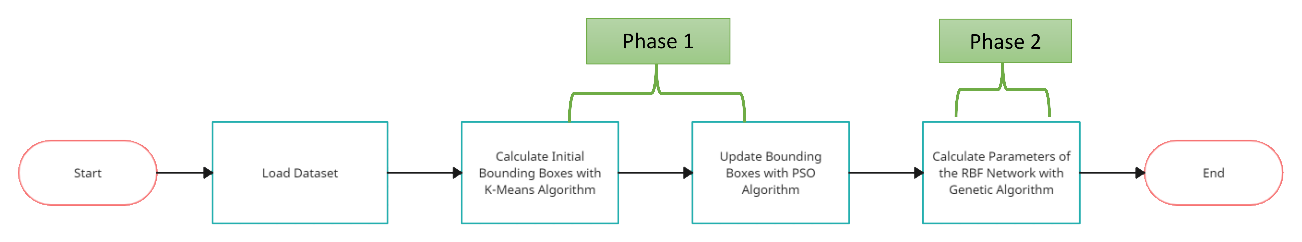
\includegraphics[scale=0.6]{datagram}
\par\end{centering}
\caption{Graphical representation of the proposed method of two phases.\label{fig:Graphical-representation-of}}

\end{figure}


\section{Experiments\label{sec:Experiments}}

The suggested method was tested on a series of classification and
regression problems found in various papers and sites from the relevant
literature. For the classification problems two internet databases
were used:
\begin{enumerate}
\item The UCI dataset repository, \url{https://archive.ics.uci.edu/ml/index.php}(accessed
on 5 January 2023)
\item The Keel repository, \url{https://sci2s.ugr.es/keel/datasets.php}(accessed
on 5 January 2023)\citep{Keel}.
\end{enumerate}
The regression datasets was found in the Statlib URL \url{ftp://lib.stat.cmu.edu/datasets/index.html }(accessed
on 5 January 2023). 

\subsection{Experimental datasets }

The classification datasets that were used are the following:
\begin{enumerate}
\item \textbf{Appendictis} dataset, a medical dataset suggested in \citep{appendicitis}.
\item \textbf{Australian} dataset \citep{australian}, an economic dataset.
\item \textbf{Balance} dataset \citep{balance}, used for prediction of
psychological states. 
\item \textbf{Cleveland} dataset, related to heart diseases \citep{cleveland1,cleveland2}.
\item \textbf{Bands} dataset, a dataset related to printing problems \citep{Bands}.
\item \textbf{Dermatology} dataset \citep{dermatology}, which is a medical
dataset.
\item \textbf{Hayes roth} dataset. This dataset\citep{hayesroth} contains
\textbf{5} numeric-valued attributes and 132 patterns. 
\item \textbf{Heart} dataset \citep{heart}, a medical dataset about heart
diseases.
\item \textbf{HouseVotes} dataset \citep{housevotes}, which is about votes
in the U.S. House of Representatives Congressmen. 
\item \textbf{Ionosphere} dataset a dataset found the Johns Hopkins database
\citep{ion1,ion2}.
\item \textbf{Liverdisorder} dataset \citep{liver}, a medical dataset about
liver disorders.
\item \textbf{Lymography} dataset \citep{lymography}. The aim here is to
detect the presence of a lymphoma in patients.
\item \textbf{Mammographic} dataset \citep{mammographic}, which is a dataset
about breast cancer.
\item \textbf{Parkinsons} dataset, a medical dataset about the Parkinson's
Disease (PD)\citep{parkinsons}.
\item \textbf{Pima} dataset, a medical dataset\citep{pima}.
\item \textbf{Popfailures} dataset \citep{popfailures}, a dataset about
climate.
\item \textbf{Spiral} dataset: The spiral artificial dataset contains 1000
two-dimensional examples that belong to two classes (500 examples
each). The number of the features is 2. The data in the first class
are created using the following formula: $x_{1}=0.5t\cos\left(0.08t\right),\ x_{2}=0.5t\cos\left(0.08t+\frac{\pi}{2}\right)$
and the second class data using\textbf{: $x_{1}=0.5t\cos\left(0.08t+\pi\right),\ x_{2}=0.5t\cos\left(0.08t+\frac{3\pi}{2}\right)$}
\item \textbf{Regions2} dataset, described in \citep{regions}. 
\item \textbf{Saheart} dataset \citep{saheart}, which is related to heart
diseases. 
\item \textbf{Segment} dataset \citep{segment}, which is related to image
processing.
\item \textbf{Wdbc} dataset \citep{wdbc}, which is related to breast tumors. 
\item \textbf{Wine} dataset. The wine recognition dataset contains data
from wine chemical analysis. It contains 178 examples of 13 features
each that are classified into three classes. It has been examinated
in many published works \citep{wine1,wine2}.
\item \textbf{Eeg} dataset. As an real word example, consider an EEG dataset
described in \citep{eeg} is used here. The datasets derived from
the dataset are denoted as Z\_F\_S, ZONF\_S and  ZO\_NF\_S.
\item \textbf{Zoo} dataset \citep{zoo}, used for classification of animals.
\end{enumerate}
The regression datasets are:
\begin{enumerate}
\item \textbf{Abalone} dataset \citep{abalone}. 
\item \textbf{Airfoil }dataset, a dataset from NASA related to aerodynamic
and acoustic tests \citep{airfoil}.
\item \textbf{Baseball} dataset, a dataset used to predict the points scored
by baseball players.
\item \textbf{BK} dataset \citep{Stat} and is used to estimate the points
scored per minute in a basketball game.
\item \textbf{BL} dataset, this dataset is related to an experiment on the
affects of machine adjustments on the time to count bolts.
\item \textbf{Concrete} dataset, related to civil engineering\citep{concrete}. 
\item \textbf{Dee} dataset, used to predict the daily average price of the
electricity energy in Spain.
\item \textbf{Diabetes} dataset, a medical dataset.
\item \textbf{FA} dataset, related to fat measurements. 
\item \textbf{Housing} dataset, described in \citep{key23}.
\item \textbf{MB} dataset, a statistics dataset \citep{key21}.
\item \textbf{MORTGAGE} dataset, which contains economic data.
\item \textbf{NT} dataset, derived from \citep{ntdataset}. 
\item \textbf{PY} dataset (Pyrimidines problem)\citep{pydataset}. 
\item \textbf{Quake} dataset, which contains data from earthquakes \citep{quake}. 
\item \textbf{Treasure} dataset, which contains economic data.
\item \textbf{Wankara} dataset, that is about weather measurement
\end{enumerate}

\subsection{Experimental results}

The RBF network for the experiments was coded in ANSI C++ with the
help of the freely available Armadillo library \citep{Armadillo}.
In addition, in order to have greater reliability in the experimental
results, a 10-fold validation technique was used. All the experiments
were executed 30 times with different seeds for the random generator
each time and the average was measured. For the classification datasets,
the average classification error was reported and for the regression
datasets the mean test error. The machine used for the experiments
was an AMD Ryzen 5950X with 128GB of RAM. The used operating system
was Debian Linux. In order to accelerate the training process, the
OpenMP library was incorporated \citep{openmp}. The experimental
settings are listed in the Table \ref{tab:Experimental-parameters}.
The experimental results for the classification datasets are listed
in Table \ref{tab:Experiments-for-classification} and for the regression
datasets in Table \ref{tab:experiments-regression}. For the experimental
tables the following are applied:
\begin{enumerate}
\item The column NN-PROP indicates the application of the Rprop method \citep{rpropnn}
in an artificial neural network \citep{nn1,nn2} with 10 hidden nodes.
The RPROP method is coded in the FCNN software package \citep{fcn}. 
\item The column NN-GENETIC denotes the application of a genetic algorithm
in the artificial neural network with 10 hidden nodes. The parameters
of the used genetic algorithm are the same as in the second phase
of the proposed method.
\item The column RBF-KMEANS denotes the classic training method for RBF
networks by estimating centers and variances through K-Means and the
output weights by solving a linear system of equations.
\item The column IRBF-100 denotes the application of the current method
with $\lambda=100$.
\item The column IRBF-1000 denotes the application of the current method
with $\lambda=1000$.
\item In both tables an extra line has been added, in which the mean error
for each method is shown. This row is denoted by the name AVERAGE.
This line also shows the number of times the corresponding method
achieved the best result. This number is shown in parentheses.
\end{enumerate}
As one can see from the experimental results, the proposed method
significantly outperforms the other techniques in the majority of
cases in terms of the average error in the test set. Moreover, the
difference from the established method of training RBF networks is
of the order of 40\% and in some cases this percentage can be doubled.
The statistical difference of the proposed technique against the rest
is also shown in graphs \ref{fig:class_error} and \ref{fig:graph_regression}.
However, the proposed technique is significantly slower than the original
training technique, as it is a two-stage technique. In the first stage,
an optimal interval of values for the network parameters is created
with a modified PSO method, and in the second stage, the network is
trained using a genetic algorithm. Of course, this extra time can
be significantly reduced by incorporating parallel techniques, as
was done experimentally using the OpenMP library. Furthermore, changing
the normalization factor $\lambda$ from 100 to 1000 did not have
much effect on the mean error in the test set. This induces that the
proposed method is quite robust, since it doesn't have much dependence
on this parameter. 

An additional experiment was performed with different values for the
parameter $F$. The experimental results for this experiment are shown
in Table \ref{tab:expsFClass} for the classification datasets and
in Table \ref{tab:expsFRegression} for the regression datasets. And
for this critical parameter, no large deviations appear in the results
of the proposed method. This further enhances the robustness and reliability
of the proposed technique.

Also, in the Table \ref{tab:precisionRecall}, the metrics of precision,
recall and f-score are shown for a series of classification datasets
and for the proposed method (mentioned as IRBF-100) and the classic
method for training RBF networks (mentioned as RBF-KMEANS) .And in
these experimental results, the reader can see the superiority of
the proposed technique over the traditional method of training RBF
networks.

\begin{table}
\caption{The used values for the experimental parameters. The first column
denotes the name of the parameter and the second the used value.\label{tab:Experimental-parameters}}

\centering{}%
\begin{tabular}{|c|c|}
\hline 
\textbf{PARAMETER} & \textbf{VALUE}\tabularnewline
\hline 
$N_{c}$ & 200\tabularnewline
\hline 
$N_{g}$ & 100\tabularnewline
\hline 
$N_{s}$ & 50\tabularnewline
\hline 
$c_{1}$ & 1.0\tabularnewline
\hline 
$c_{2}$ & 1.0\tabularnewline
\hline 
$F$ & 5.0\tabularnewline
\hline 
$B$ & 100.0\tabularnewline
\hline 
$k$ & 10\tabularnewline
\hline 
$p_{s}$ & 0.90\tabularnewline
\hline 
$p_{m}$ & 0.05\tabularnewline
\hline 
\end{tabular}
\end{table}

\begin{table}
\caption{Experimental results for the classification datasets. The first column
is the name of the used dataset.\label{tab:Experiments-for-classification}}

\centering{}%
\begin{tabular}{|c|c|c|c|c|c|}
\hline 
DATASET & NN-RPROP & NN-GENETIC & RBF-KMEANS & IRBF-100 & IRBF-1000\tabularnewline
\hline 
\hline 
Appendicitis & 16.30\% & 18.10\% & \textbf{12.23\%} & 16.47\% & 14.03\%\tabularnewline
\hline 
Australian & 36.12\% & 32.21\% & 34.89\% & 23.61\% & \textbf{22.39\%}\tabularnewline
\hline 
Balance & \textbf{8.81\%} & 8.97\% & 33.42\% & 12.65\% & 13.15\%\tabularnewline
\hline 
Bands & 36.32\% & \textbf{35.75\%} & 37.22\% & 37.38\% & 36.29\%\tabularnewline
\hline 
Cleveland & 61.41\% & 51.60\% & 67.10\% & 49.77\% & \textbf{49.64\%}\tabularnewline
\hline 
Dermatology & \textbf{15.12\%} & 30.58\% & 62.34\% & 38.24\% & 35.64\%\tabularnewline
\hline 
Hayes Roth & 37.46\% & 56.18\% & 64.36\% & \textbf{33.62\%} & 34.13\%\tabularnewline
\hline 
Heart & 30.51\% & 28.34\% & 31.20\% & 15.91\% & \textbf{15.60\%}\tabularnewline
\hline 
HouseVotes & 6.04\% & 6.62\% & 6.13\% & 4.77\% & \textbf{3.90\%}\tabularnewline
\hline 
Ionosphere & 13.65\% & 15.14\% & 16.22\% & 8.64\% & \textbf{7.52\%}\tabularnewline
\hline 
Liverdisorder & 40.26\% & 31.11\% & 30.84\% & 27.36\% & \textbf{25.63\%}\tabularnewline
\hline 
Lymography & 24.67\% & 23.26\% & 25.31\% & \textbf{19.12\%} & 20.02\%\tabularnewline
\hline 
Mammographic & 18.46\% & 19.88\% & 21.38\% & \textbf{17.17\%} & 17.30\%\tabularnewline
\hline 
Parkinsons & 22.28\% & 18.05\% & 17.41\% & 15.51\% & \textbf{13.59\%}\tabularnewline
\hline 
Pima & 34.27\% & 32.19\% & 25.78\% & 23.61\% & \textbf{23.23\%}\tabularnewline
\hline 
Popfailures & \textbf{4.81\%} & 5.94\% & 7.04\% & 5.21\% & 5.10\%\tabularnewline
\hline 
Regions2 & 27.53\% & 29.39\% & 38.29\% & 26.08\% & \textbf{25.77\%}\tabularnewline
\hline 
Saheart & 34.90\% & 34.86\% & 32.19\% & \textbf{27.94\%} & 28.91\%\tabularnewline
\hline 
Segment & 52.14\% & 57.72\% & 59.68\% & 47.19\% & \textbf{40.28\%}\tabularnewline
\hline 
Spiral & 46.59\% & 44.50\% & 44.87\% & \textbf{19.43\%} & 19.56\%\tabularnewline
\hline 
Wdbc & 21.57\% & 8.56\% & 7.27\% & \textbf{5.33\%} & 5.44\%\tabularnewline
\hline 
Wine & 30.73\% & 19.20\% & 31.41\% & 9.20\% & \textbf{6.84\%}\tabularnewline
\hline 
Z\_F\_S & 29.28\% & 10.73\% & 13.16\% & 4.19\% & \textbf{4.18\%}\tabularnewline
\hline 
ZO\_NF\_S & 6.43\% & 8.41\% & 9.02\% & \textbf{4.31\%} & 4.35\%\tabularnewline
\hline 
ZONF\_S & 27.27\% & 2.60\% & 4.03\% & 2.23\% & \textbf{2.08\%}\tabularnewline
\hline 
ZOO & 15.47\% & 16.67\% & 21.93\% & \textbf{10.13\%} & 11.13\%\tabularnewline
\hline 
\textbf{AVERAGE} & \textbf{26.86\%(3)} & \textbf{24.87\%(1)} & \textbf{29.03\%(1)} & \textbf{19.43\%(8)} & \textbf{18.68\%(13)}\tabularnewline
\hline 
\end{tabular}
\end{table}
\begin{table}
\caption{Experimental results for the regression datasets. The first column
is the name of the used regression dataset.\label{tab:experiments-regression}}

\centering{}%
\begin{tabular}{|c|c|c|c|c|c|}
\hline 
\textbf{DATASET} & \textbf{NN-RPROP} & \textbf{NN-GENETIC} & \textbf{RBF-KMEANS} & \textbf{IRBF-100} & \textbf{IRBF-1000}\tabularnewline
\hline 
ABALONE & \textbf{4.55} & 7.17 & 7.37 & 5.57 & 5.32\tabularnewline
\hline 
AIRFOIL & 0.002 & 0.003 & 0.27 & 0.004 & \textbf{0.003}\tabularnewline
\hline 
BASEBALL & 92.05 & 103.60 & 93.02 & \textbf{78.89} & 85.58\tabularnewline
\hline 
BK & 1.60 & 0.03 & \textbf{0.02} & 0.04 & 0.03\tabularnewline
\hline 
BL & 4.38 & 5.74 & 0.013 & \textbf{0.0003} & 0.0003\tabularnewline
\hline 
CONCRETE & 0.009 & 0.009 & 0.011 & \textbf{0.007} & 0.007\tabularnewline
\hline 
DEE & 0.608 & 1.013 & 0.17 & \textbf{0.16} & 0.16\tabularnewline
\hline 
DIABETES & 1.11 & 19.86 & \textbf{0.49} & 0.78 & 0.89\tabularnewline
\hline 
HOUSING & 74.38 & 43.26 & 57.68 & \textbf{20.27} & 21.54\tabularnewline
\hline 
FA & 0.14 & 1.95 & \textbf{0.015} & 0.032 & 0.029\tabularnewline
\hline 
MB & 0.55 & 3.39 & 2.16 & 0.12 & \textbf{0.09}\tabularnewline
\hline 
MORTGAGE & 9.19 & 2.41 & 1.45 & \textbf{0.39} & 0.78\tabularnewline
\hline 
NT & 0.04 & \textbf{0.006} & 8.14 & 0.007 & 0.007\tabularnewline
\hline 
PY & 0.039 & 1.41 & \textbf{0.012} & 0.024 & 0.014\tabularnewline
\hline 
QUAKE & 0.041 & 0.040 & 0.07 & 0.04 & \textbf{0.03}\tabularnewline
\hline 
TREASURY & 10.88 & 2.93 & 2.02 & \textbf{0.33} & 0.51\tabularnewline
\hline 
WANKARA & 0.0003 & 0.012 & \textbf{0.001} & 0.002 & 0.002\tabularnewline
\hline 
\textbf{AVERAGE} & \textbf{11.71(1)} & \textbf{11.34(1)} & \textbf{10.17(5)} & \textbf{6.27(7)} & \textbf{6.76(3)}\tabularnewline
\hline 
\end{tabular}
\end{table}
\begin{figure}[H]
\centering{}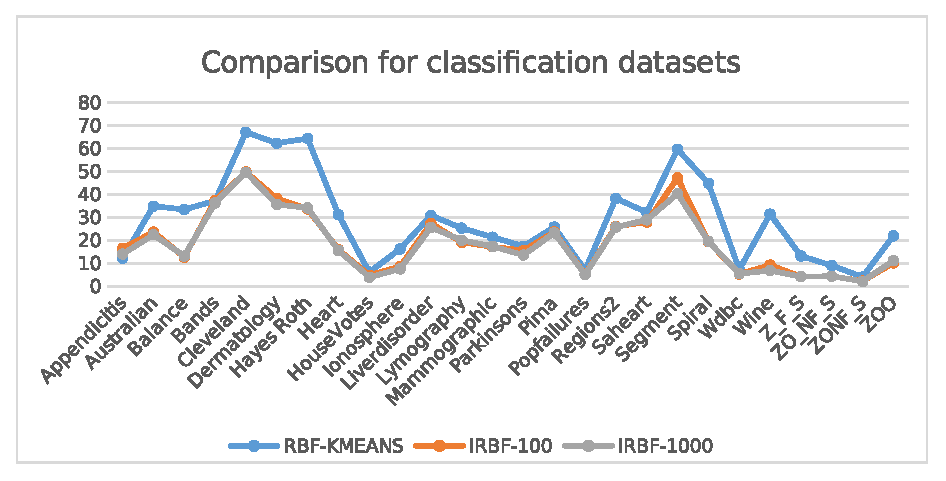
\includegraphics[scale=0.7]{classcomparison}\caption{Graphical comparison of all methods for the classification datasets.
\label{fig:class_error}}
\end{figure}
\begin{figure}[H]
\centering{}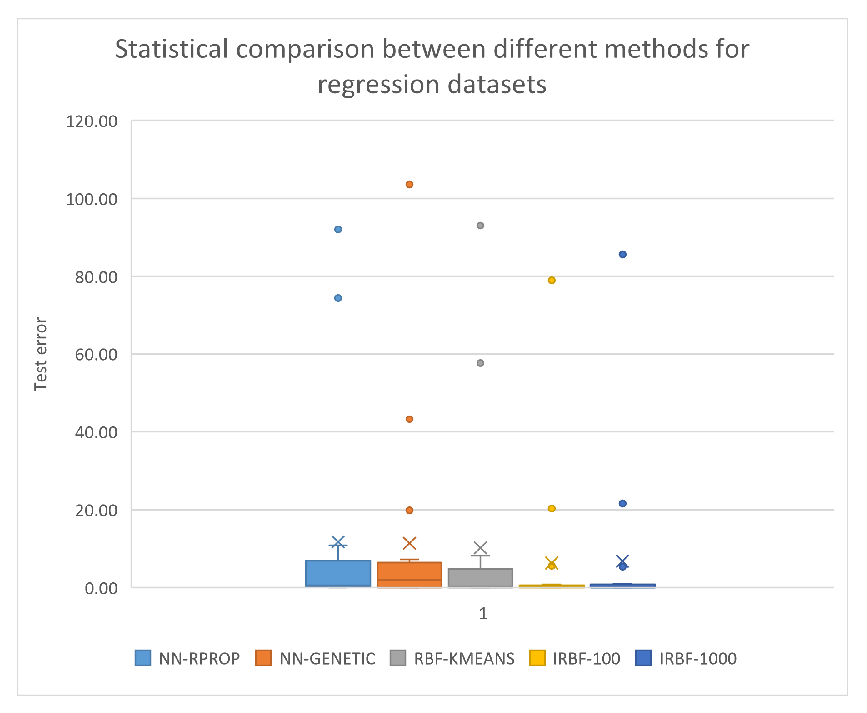
\includegraphics[scale=0.7]{regression_comparison}\caption{Graphical comparison of the methods for the regression datasets.\label{fig:graph_regression}}
\end{figure}

\begin{table}[H]
\caption{Experimental results with the proposed method and using different
values for the parameter $F$ on the classification datasets.\label{tab:expsFClass}}

\centering{}%
\begin{tabular}{|c|c|c|c|}
\hline 
\textbf{DATASET} & \textbf{$F=3$} & \textbf{$F=5$} & \textbf{$F=10$}\tabularnewline
\hline 
Appendicitis & 14.43\% & 14.03\% & 14.47\%\tabularnewline
\hline 
Australian & 23.45\% & 22.39\% & 23.21\%\tabularnewline
\hline 
Balance & 13.35\% & 13.15\% & 11.79\%\tabularnewline
\hline 
Bands & 36.48\% & 36.29\% & 36.76\%\tabularnewline
\hline 
Cleveland & 49.26\% & 49.64\% & 49.02\%\tabularnewline
\hline 
Dermatology & 36.54\% & 35.64\% & 34.37\%\tabularnewline
\hline 
Hayes Roth & 39.28\% & 34.13\% & 36.46\%\tabularnewline
\hline 
Heart & 15.14\% & 15.60\% & 14.89\%\tabularnewline
\hline 
HouseVotes & 4.93\% & 3.90\% & 6.41\%\tabularnewline
\hline 
Ionosphere & 7.56\% & 7.52\% & 9.05\%\tabularnewline
\hline 
Liverdisorder & 28.37\% & 25.63\% & 28.97\%\tabularnewline
\hline 
Lymography & 20.12\% & 20.02\% & 21.05\%\tabularnewline
\hline 
Mammographic & 18.04\% & 17.30\% & 18.21\%\tabularnewline
\hline 
Parkinsons & 18.51\% & 13.59\% & 13.49\%\tabularnewline
\hline 
Pima & 23.69\% & 23.23\% & 23.52\%\tabularnewline
\hline 
Popfailures & 5.76\% & 5.10\% & 4.50\%\tabularnewline
\hline 
Regions2 & 25.79\% & 25.77\% & 25.32\%\tabularnewline
\hline 
Saheart & 28.89\% & 28.91\% & 26.99\%\tabularnewline
\hline 
Segment & 36.53\% & 40.28\% & 43.28\%\tabularnewline
\hline 
Spiral & 16.78\% & 19.56\% & 22.18\%\tabularnewline
\hline 
Wdbc & 4.64\% & 5.44\% & 5.10\%\tabularnewline
\hline 
Wine & 8.31\% & 6.84\% & 8.27\%\tabularnewline
\hline 
Z\_F\_S & 4.32\% & 4.18\% & 4.03\%\tabularnewline
\hline 
ZO\_NF\_S & 3.70\% & 4.35\% & 3.72\%\tabularnewline
\hline 
ZONF\_S & 2.04\% & 2.08\% & 1.98\%\tabularnewline
\hline 
ZOO & 11.87\% & 11.13\% & 9.97\%\tabularnewline
\hline 
\textbf{AVERAGE} & \textbf{18.65\%} & \textbf{18.68\%} & \textbf{19.12\%}\tabularnewline
\hline 
\end{tabular}
\end{table}
\begin{table}[H]
\caption{Experimental results with the proposed method using different values
for the parameter $F$ on the classification datasets.\label{tab:expsFRegression}}

\centering{}%
\begin{tabular}{|c|c|c|c|}
\hline 
\textbf{DATASET} & \textbf{$F=3$} & \textbf{$F=5$} & \textbf{$F=10$}\tabularnewline
\hline 
ABALONE & 5.56 & 5.32 & 5.41\tabularnewline
\hline 
AIRFOIL & 0.004 & 0.003 & 0.004\tabularnewline
\hline 
BASEBALL & 88.40 & 85.58 & 84.43\tabularnewline
\hline 
BK & 0.03 & 0.03 & 0.02\tabularnewline
\hline 
BL & 0.0005 & 0.0003 & 0.0002\tabularnewline
\hline 
CONCRETE & 0.009 & 0.007 & 0.007\tabularnewline
\hline 
DEE & 0.18 & 0.16 & 0.16\tabularnewline
\hline 
DIABETES & 0.67 & 0.89 & 0.77\tabularnewline
\hline 
HOUSING & 20.03 & 21.54 & 20.84\tabularnewline
\hline 
FA & 0.03 & 0.029 & 0.036\tabularnewline
\hline 
MB & 0.19 & 0.09 & 0.26\tabularnewline
\hline 
MORTGAGE & 0.89 & 0.78 & 0.03\tabularnewline
\hline 
NT & 0.006 & 0.007 & 0.007\tabularnewline
\hline 
PY & 0.027 & 0.014 & 0.018\tabularnewline
\hline 
QUAKE & 0.04 & 0.03 & 0.04\tabularnewline
\hline 
TREASURY & 0.77 & 0.51 & 0.17\tabularnewline
\hline 
WANKARA & 0.002 & 0.002 & 0.002\tabularnewline
\hline 
\textbf{AVERAGE} & \textbf{6.87} & \textbf{6.76} & \textbf{6.60}\tabularnewline
\hline 
\end{tabular}
\end{table}
\begin{table}[H]

\caption{Precision, recall and f-score for a series of classification datasets.\label{tab:precisionRecall}}

\centering{}%
\begin{tabular}{|c|c|}
\hline 
{\footnotesize{}RBF-KMEANS} & {\footnotesize{}IRBF-100}\tabularnewline
\hline 
\hline 
{\footnotesize{}}%
\begin{tabular}{|c|c|c|c|}
\hline 
{\footnotesize{}DATASET} & {\footnotesize{}PRECISION} & {\footnotesize{}RECALL} & {\footnotesize{}F-SCORE}\tabularnewline
\hline 
\hline 
{\footnotesize{}APPENDICITIS} & {\footnotesize{}0.80} & {\footnotesize{}0.77} & {\footnotesize{}0.76}\tabularnewline
\hline 
{\footnotesize{}AUSTRALIAN} & {\footnotesize{}0.67} & {\footnotesize{}0.61} & {\footnotesize{}0.58}\tabularnewline
\hline 
{\footnotesize{}BALANCE} & {\footnotesize{}0.74} & {\footnotesize{}0.76} & {\footnotesize{}0.64}\tabularnewline
\hline 
{\footnotesize{}BANDS} & {\footnotesize{}0.52} & {\footnotesize{}0.51} & {\footnotesize{}0.48}\tabularnewline
\hline 
{\footnotesize{}HEART} & {\footnotesize{}0.68} & {\footnotesize{}0.69} & {\footnotesize{}0.67}\tabularnewline
\hline 
{\footnotesize{}IONOSPHERE} & {\footnotesize{}0.84} & {\footnotesize{}0.81} & {\footnotesize{}0.81}\tabularnewline
\hline 
{\footnotesize{}LIVERDISORDER} & {\footnotesize{}0.65} & {\footnotesize{}0.64} & {\footnotesize{}0.64}\tabularnewline
\hline 
{\footnotesize{}MAMMOGRAPHIC} & {\footnotesize{}0.81} & {\footnotesize{}0.81} & {\footnotesize{}0.81}\tabularnewline
\hline 
{\footnotesize{}PARKINSONS} & {\footnotesize{}0.76} & {\footnotesize{}0.68} & {\footnotesize{}0.69}\tabularnewline
\hline 
{\footnotesize{}PIMA} & {\footnotesize{}0.72} & {\footnotesize{}0.67} & {\footnotesize{}0.68}\tabularnewline
\hline 
{\footnotesize{}SAHEART} & {\footnotesize{}0.65} & {\footnotesize{}0.61} & {\footnotesize{}0.61}\tabularnewline
\hline 
{\footnotesize{}SEGMENT} & {\footnotesize{}0.43} & {\footnotesize{}0.39} & {\footnotesize{}0.39}\tabularnewline
\hline 
{\footnotesize{}SPIRAL} & {\footnotesize{}0.56} & {\footnotesize{}0.56} & {\footnotesize{}0.55}\tabularnewline
\hline 
{\footnotesize{}WDBC} & {\footnotesize{}0.93} & {\footnotesize{}0.91} & {\footnotesize{}0.92}\tabularnewline
\hline 
{\footnotesize{}WINE} & {\footnotesize{}0.74} & {\footnotesize{}0.65} & {\footnotesize{}0.66}\tabularnewline
\hline 
{\footnotesize{}Z\_F\_S} & {\footnotesize{}0.85} & {\footnotesize{}0.84} & {\footnotesize{}0.83}\tabularnewline
\hline 
{\footnotesize{}ZO\_NF\_S} & {\footnotesize{}0.90} & {\footnotesize{}0.90} & {\footnotesize{}0.90}\tabularnewline
\hline 
\end{tabular} & {\footnotesize{}}%
\begin{tabular}{|c|c|c|}
\hline 
{\footnotesize{}PRECISION} & {\footnotesize{}RECALL} & {\footnotesize{}F-SCORE}\tabularnewline
\hline 
\hline 
{\footnotesize{}0.79} & {\footnotesize{}0.74} & {\footnotesize{}0.78}\tabularnewline
\hline 
{\footnotesize{}0.79} & {\footnotesize{}0.76} & {\footnotesize{}0.76}\tabularnewline
\hline 
{\footnotesize{}0.75} & {\footnotesize{}0.78} & {\footnotesize{}0.76}\tabularnewline
\hline 
{\footnotesize{}0.58} & {\footnotesize{}0.57} & {\footnotesize{}0.56}\tabularnewline
\hline 
{\footnotesize{}0.86} & {\footnotesize{}0.85} & {\footnotesize{}0.85}\tabularnewline
\hline 
{\footnotesize{}0.92} & {\footnotesize{}0.89} & {\footnotesize{}0.90}\tabularnewline
\hline 
{\footnotesize{}0.72} & {\footnotesize{}0.71} & {\footnotesize{}0.71}\tabularnewline
\hline 
{\footnotesize{}0.83} & {\footnotesize{}0.83} & {\footnotesize{}0.82}\tabularnewline
\hline 
{\footnotesize{}0.85} & {\footnotesize{}0.80} & {\footnotesize{}0.81}\tabularnewline
\hline 
{\footnotesize{}0.75} & {\footnotesize{}0.70} & {\footnotesize{}0.71}\tabularnewline
\hline 
{\footnotesize{}0.70} & {\footnotesize{}0.66} & {\footnotesize{}0.67}\tabularnewline
\hline 
{\footnotesize{}0.58} & {\footnotesize{}0.53} & {\footnotesize{}0.53}\tabularnewline
\hline 
{\footnotesize{}0.70} & {\footnotesize{}0.70} & {\footnotesize{}0.70}\tabularnewline
\hline 
{\footnotesize{}0.96} & {\footnotesize{}0.94} & {\footnotesize{}0.95}\tabularnewline
\hline 
{\footnotesize{}0.93} & {\footnotesize{}0.93} & {\footnotesize{}0.92}\tabularnewline
\hline 
{\footnotesize{}0.96} & {\footnotesize{}0.97} & {\footnotesize{}0.96}\tabularnewline
\hline 
{\footnotesize{}0.95} & {\footnotesize{}0.95} & {\footnotesize{}0.95}\tabularnewline
\hline 
\end{tabular}\tabularnewline
\hline 
\end{tabular}
\end{table}


\section{Conclusions\label{sec:Conclusions}}

In the present work, a two-stage hybrid method was proposed to efficiently
identify the parameters of RBF neural networks. In the first stage
of the method, a technique rooted in particle swarm optimization was
used to efficiently identify a reliable interval of values for the
neural network parameters. In the second stage of the method, an intelligent
global optimization technique was used to locate the neural network
parameters within the optimal value interval of the first stage. In
this work, a genetic algorithm was used in the second phase, but any
global optimization method could be used in its place.

The method was applied to a multitude of classification and regression
problems from the relevant literature. In almost all cases, the proposed
method significantly outperforms other machine learning models, and
on average the improvement in the error on the test sets was of the
order of 40\% relative to the established RBF training method. Moreover,
the method is quite robust with respect to the basic parameters since
any changes in the parameter values do not significantly affect its
performance. Furthermore, the method can efficiently locate the value
interval of network parameters without any prior knowledge about the
type of training data or whether it is a classification or a regression
problem. However, the proposed technique is significantly more time-consuming
than the traditional training technique as it requires computational
time for both its phases. Although, this effect can be overcomed to
some extent by the use of modern parallel computing techniques.

The method could be extended by the use of other techniques of training
the parameters in RBF networks, such as, for example, the differential
evolutionary method \citep{dePaper}. Furthermore, more efficient
methods of terminating the first stage of the method could be used
as finding a suitable interval of values for the network parameters
requires many numerical calculations.

\vspace{6pt}


\authorcontributions{I.G.T. and V.C. conceived of the idea and methodology and supervised
the technical part regarding the software. I.G.T. conducted the experiments,
employing datasets, and provided the comparative experiments. V.C.
performed the statistical analysis and prepared the manuscript. All
authors have read and agreed to the published version of the manuscript.}

\funding{This research received no external funding.}

\institutionalreview{Not applicable.}

\informedconsent{Not applicable. }

\institutionalreview{Not applicable.}

\acknowledgments{The experiments of this research work were performed at the high
performance computing system established at Knowledge and Intelligent
Computing Laboratory, Department of Informatics and Telecommunications,
University of Ioannina, acquired with the project “Educational Laboratory
equipment of TEI of Epirus” with MIS 5007094 funded by the Operational
Programme “Epirus” 2014--2020, by ERDF and national funds.}

\conflictsofinterest{The authors declare no conflict of interest.}

\sampleavailability{Not applicable.}

\appendixtitles{no}

\appendixstart{}

\begin{adjustwidth}{-\extralength}{0cm}{}


\reftitle{References}
\begin{thebibliography}{999}
\bibitem{physics_ml1} M. Mjahed, The use of clustering techniques
for the classification of high energy physics data, Nuclear Instruments
and Methods in Physics Research Section A: Accelerators, Spectrometers,
Detectors and Associated Equipment \textbf{559}, pp. 199-202, 2006.

\bibitem{physics_ml2}M Andrews, M Paulini, S Gleyzer, B Poczos, End-to-End
Event Classification of High-Energy Physics Data, Journal of Physics:
Conference Series \textbf{1085}, 2018.

\bibitem{chemistry_ml1}P. He, C.J. Xu, Y.Z. Liang, K.T. Fang, Improving
the classification accuracy in chemistry via boosting technique, Chemometrics
and Intelligent Laboratory Systems 70, pp. 39-46, 2004.

\bibitem{chemistry_ml2}J.A. Aguiar, M.L. Gong, T.Tasdizen, Crystallographic
prediction from diffraction and chemistry data for higher throughput
classification using machine learning, Computational Materials Science
\textbf{173}, 109409, 2020.

\bibitem{econ_ml1}I. Kaastra, M. Boyd, Designing a neural network
for forecasting financial and economic time series, Neurocomputing
\textbf{10}, pp. 215-236, 1996.

\bibitem{econ_ml2}R. Hafezi, J. Shahrabi, E. Hadavandi, A bat-neural
network multi-agent system (BNNMAS) for stock price prediction: Case
study of DAX stock price, Applied Soft Computing \textbf{29}, pp.
196-210, 2015.

\bibitem{med_ml1}S.S. Yadav, S.M. Jadhav, Deep convolutional neural
network based medical image classification for disease diagnosis.
J Big Data \textbf{6}, 113, 2019.

\bibitem{med_ml2}L. Qing, W. Linhong , D. Xuehai, A Novel Neural
Network-Based Method for Medical Text Classification, Future Internet
\textbf{11}, 255, 2019. 

\bibitem{rbf1}J. Park and I. W. Sandberg, Universal Approximation
Using Radial-Basis-Function Networks, Neural Computation \textbf{3},
pp. 246-257, 1991.

\bibitem{rbfghosh}J. Ghosh, A. Nag, An Overview of Radial Basis Function
Networks. In: Howlett, R.J., Jain, L.C. (eds) Radial Basis Function
Networks 2. Studies in Fuzziness and Soft Computing, vol 67. Physica,
Heidelberg, 2001.

\bibitem{rbfde1}Nam Mai-Duy, Thanh Tran-Cong, Numerical solution
of differential equations using multiquadric radial basis function
networks, Neural Networks 14, pp. 185-199, 2001.

\bibitem{rbfde2}N. Mai‐Duy, Solving high order ordinary differential
equations with radial basis function networks. Int. J. Numer. Meth.
Engng. \textbf{62}, pp. 824-852, 2005.

\bibitem{rbfnetwork1}C. Laoudias, P. Kemppi and C. G. Panayiotou,
Localization Using Radial Basis Function Networks and Signal Strength
Fingerprints in WLAN, GLOBECOM 2009 - 2009 IEEE Global Telecommunications
Conference, Honolulu, HI, 2009, pp. 1-6, 2009.

\bibitem{rbfnetwork2}M. Azarbad, S. Hakimi, A. Ebrahimzadeh, Automatic
recognition of digital communication signal, International journal
of energy, information and communications \textbf{3}, pp. 21-33, 2012.

\bibitem{rbfphysics1}P. Teng, Machine-learning quantum mechanics:
Solving quantum mechanics problems using radial basis function networks,
Phys. Rev. E \textbf{98}, 033305, 2018.

\bibitem{rbfphysics2}R. Jovanović, A. Sretenovic, Ensemble of radial
basis neural networks with K-means clustering for heating energy consumption
prediction, FME Transactions \textbf{45}, pp. 51-57, 2017.

\bibitem{rbfchemistry1}D.L. Yu, J.B. Gomm, D. Williams, Sensor fault
diagnosis in a chemical process via RBF neural networks, Control Engineering
Practice \textbf{7}, pp. 49-55, 1999.

\bibitem{rbfchemistry2}V. Shankar, G.B. Wright, A.L. Fogelson, R.M.
Kirby, A radial basis function (RBF) finite difference method for
the simulation of reaction--diffusion equations on stationary platelets
within the augmented forcing method, Int. J. Numer. Meth. Fluids \textbf{75},
pp. 1-22, 2014.

\bibitem{rbfecon0}W. Shen, X. Guo, C. Wu, D. Wu, Forecasting stock
indices using radial basis function neural networks optimized by artificial
fish swarm algorithm, Knowledge-Based Systems 24, pp. 378-385, 2011.

\bibitem{rbfecon1}J. A. Momoh, S. S. Reddy, Combined Economic and
Emission Dispatch using Radial Basis Function, 2014 IEEE PES General
Meeting \textbar{} Conference \& Exposition, National Harbor, MD,
pp. 1-5, 2014.

\bibitem{rbfecon2}P. Sohrabi, B. Jodeiri Shokri, H. Dehghani, Predicting
coal price using time series methods and combination of radial basis
function (RBF) neural network with time series. Miner Econ 2021.

\bibitem{rbf_dos1}U. Ravale, N. Marathe, P. Padiya, Feature Selection
Based Hybrid Anomaly Intrusion Detection System Using K Means and
RBF Kernel Function, Procedia Computer Science \textbf{45}, pp. 428-435,
2015.

\bibitem{rbf_dos2}M. Lopez-Martin, A. Sanchez-Esguevillas, J. I.
Arribas, B. Carro, Network Intrusion Detection Based on Extended RBF
Neural Network With Offline Reinforcement Learning, IEEE Access \textbf{9},
pp. 153153-153170, 2021.

\bibitem{rbfadv}H. Yu, T. Xie, S. Paszczynski and B. M. Wilamowski,
Advantages of Radial Basis Function Networks for Dynamic System Design,IEEE
Transactions on Industrial Electronics v\textbf{ 58}, pp. 5438-5450,
2011.

\bibitem{rbfpar1}R. Yokota, L.A. Barba, M. G. Knepley, PetRBF ---
A parallel O(N) algorithm for radial basis function interpolation
with Gaussians, Computer Methods in Applied Mechanics and Engineering
\textbf{199}, pp. 1793-1804, 2010.

\bibitem{rbfpar2}C. Lu, N. Ma, Z. Wang, Fault detection for hydraulic
pump based on chaotic parallel RBF network, EURASIP J. Adv. Signal
Process. \textbf{2011}, 49, 2011.

\bibitem{rbfinit1}L.I. Kuncheva, Initializing of an RBF network by
a genetic algorithm, Neurocomputing \textbf{14}, pp. 273-288, 1997.

\bibitem{rbfinit2}F. Ros, M. Pintore, A. Deman, J.R. Chrétien, Automatical
initialization of RBF neural networks, Chemometrics and Intelligent
Laboratory Systems \textbf{87}, pp. 26-32, 2007.

\bibitem{rbfinit3}D. Wang, X.J. Zeng, J.A. Keane, A clustering algorithm
for radial basis function neural network initialization, Neurocomputing
\textbf{77}, pp. 144-155, 2012.

\bibitem{rbfprun1}E. Ricci, R. Perfetti, Improved pruning strategy
for radial basis function networks with dynamic decay adjustment,
Neurocomputing \textbf{69}, pp. 1728-1732, 2006.

\bibitem{rbfprun3}Guang-Bin Huang, P. Saratchandran and N. Sundararajan,
A generalized growing and pruning RBF (GGAP-RBF) neural network for
function approximation, IEEE Transactions on Neural Networks \textbf{16},
pp. 57-67, 2005.

\bibitem{rbfprun2}M. Bortman and M. Aladjem, A Growing and Pruning
Method for Radial Basis Function Networks, IEEE Transactions on Neural
Networks \textbf{20}, pp. 1039-1045, 2009.

\bibitem{rbfcon1}N. B. Karayiannis, M. M. Randolph-Gips, On the construction
and training of reformulated radial basis function neural networks,
IEEE Transactions on Neural Networks \textbf{14}, pp. 835-846, 2003.

\bibitem{rbfcon2}J.X. Peng, K. Li, D.S. Huang, A Hybrid Forward Algorithm
for RBF Neural Network Construction, IEEE Transactions on Neural Networks,
\textbf{17}, pp. 1439-1451, 2006.

\bibitem{rbfcon3}D. Du, K. Li, M. Fei, A fast multi-output RBF neural
network construction method, Neurocomputing \textbf{73}, pp. 2196-2202,
2010.

\bibitem{rbftune}V. Agarwal, S. Bhanot, Radial basis function neural
network-based face recognition using firefly algorithm, Neural Comput
\& Applic \textbf{30}, pp. 2643--2660, 2018.

\bibitem{rbfABC}S. Jiang et al., Prediction of Ecological Pressure
on Resource-Based Cities Based on an RBF Neural Network Optimized
by an Improved ABC Algorithm, IEEE Access.\textbf{ 7}, pp. 47423-47436,
2019.

\bibitem{psoTutorial}F. Marini, B. Walczak, Particle swarm optimization
(PSO). A tutorial, Chemometrics and Intelligent Laboratory Systems
\textbf{149}, pp. 153-165, 2015.

\bibitem{psoApp1}B. Liu, L. Wang, Y.H. Jin, An Effective PSO-Based
Memetic Algorithm for Flow Shop Scheduling, IEEE Transactions on Systems,
Man, and Cybernetics, Part B (Cybernetics) \textbf{37}, pp. 18-27,
2007.

\bibitem{psoApp2}J. Yang, L. He, S. Fu, An improved PSO-based charging
strategy of electric vehicles in electrical distribution grid, Applied
Energy \textbf{128}, pp. 82-92, 2014.

\bibitem{psoApp3}K. Mistry, L. Zhang, S. C. Neoh, C. P. Lim, B. Fielding,
A Micro-GA Embedded PSO Feature Selection Approach to Intelligent
Facial Emotion Recognition, IEEE Transactions on Cybernetics. \textbf{47},
pp. 1496-1509, 2017.

\bibitem{psoApp4}S. Han, X. Shan, J. Fu, W. Xu, H. Mi, Industrial
robot trajectory planning based on improved pso algorithm, J. Phys.:
Conf. Ser. \textbf{1820}, 012185, 2021.

\bibitem{goReview}C.A. Floudas, C.E. Gounaris, A review of recent
advances in global optimization, J Glob Optim \textbf{45}, pp. 3--38,
2009.

\bibitem{fireflyMain}H. Wang, W. Wang, X. Zhou, H. Sun, J. Zhao,
X. Yu, Z. Cui, Firefly algorithm with neighborhood attraction, Information
Sciences \textbf{382-383}, pp. 374-387, 2017.

\bibitem{ga1}D. Goldberg, Genetic Algorithms in Search, Optimization
and Machine Learning, Addison-Wesley Publishing Company, Reading,
Massachussets, 1989.

\bibitem{ga2}Z. Michaelewicz, Genetic Algorithms + Data Structures
= Evolution Programs. Springer - Verlag, Berlin, 1996.

\bibitem{ga3}S.A. Grady, M.Y. Hussaini, M.M. Abdullah, Placement
of wind turbines using genetic algorithms, Renewable Energy \textbf{30},
pp. 259-270, 2005.

\bibitem{fireflyCancer}I.U. Khan,N. Aslam, R. Alshehri, S. Alzahrani,
M. Alghamdi, A. Almalki, M. Balabeed, Cervical Cancer Diagnosis Model
Using Extreme Gradient Boosting and Bioinspired Firefly Optimization,
Scientific Programming \textbf{2021}, Article ID 5540024, 2021.

\bibitem{hybridCNN}M. Zivkovic, N. Bacanin, M. Antonijevic, B. Nikolic,
G. Kvascev, M. Marjanovic, N. Savanovic, Hybrid CNN and XGBoost Model
Tuned by Modified Arithmetic Optimization Algorithm for COVID-19 Early
Diagnostics from X-ray Images, Electronics \textbf{11}, 3798, 2022.

\bibitem{kmeans}J. MacQueen, Some methods for classification and
analysis of multivariate observations, in: Proceedings of the fifth
Berkeley symposium on mathematical statistics and probability, Vol.
1, No. 14, pp. 281-297, 1967. 

\bibitem{interval0}E. Hansen and G.W. Walster.Global Optimization
using Interval Analy-sis.Marcel Dekker Inc., New York, 2004.

\bibitem{interval1}M. Markót, J. Fernández, L. Casado et al, New
interval methods for constrained global optimization, Mathematical
Programming \textbf{106}, pp. 287-318, 2006.

\bibitem{interval2}A. Žilinskas, J. Žilinskas, Interval Arithmetic
Based Optimization in Nonlinear Regression, Informatica \textbf{21},
pp. 149-158, 2010.

\bibitem{interval_app1}C.A. Schnepper, M.A. Stadtherr, Robust process
simulation using interval methods, Computers \& Chemical Engineering
\textbf{20}, pp. 187-199, 1996.

\bibitem{interval_app2}C. Carreras, I. D. Walker, Interval methods
for fault-tree analysis in robotics, IEEE Transactions on Reliability
\textbf{50}, pp. 3-11, 2001.

\bibitem{interval_app3}A. Serguieva, J. Hunte, Fuzzy interval methods
in investment risk appraisal, Fuzzy Sets and Systems \textbf{142},
pp. 443-466, 2004.

\bibitem{pso1}Riccardo Poli, James Kennedy kennedy, Tim Blackwell,
Particle swarm optimization An Overview, Swarm Intelligence \textbf{1},
pp 33-57, 2007. 

\bibitem{psoConstant}I.C. Trelea, The particle swarm optimization
algorithm: convergence analysis and parameter selection, Information
Processing Letters \textbf{85}, pp. 317-325, 2003.

\bibitem{psoLinear}Y. Shi, R.C. Eberhart, Empirical study of particle
swarm optimization, In: Proceedings of the 1999 Congress on Evolutionary
Computation-CEC99 (Cat. No. 99TH8406), pp. 1945-1950 Vol. 3, 1999.

\bibitem{psoExp}B. Borowska, Exponential Inertia Weight in Particle
Swarm Optimization. In: Wilimowska, Z., Borzemski, L., Grzech, A.,
Świątek, J. (eds) Information Systems Architecture and Technology:
Proceedings of 37th International Conference on Information Systems
Architecture and Technology -- ISAT 2016 -- Part IV. Advances in
Intelligent Systems and Computing, vol 524. Springer, Cham, 2017.

\bibitem{psoRandom}L. Zhang, H. Yu, S. Hu, A New Approach to Improve
Particle Swarm Optimization. In: , et al. Genetic and Evolutionary
Computation --- GECCO 2003. GECCO 2003. Lecture Notes in Computer
Science, vol 2723. Springer, Berlin, Heidelberg, 2003.

\bibitem{psoDynamic}B. Borowska, Dynamic Inertia Weight in Particle
Swarm Optimization. In: Shakhovska, N., Stepashko, V. (eds) Advances
in Intelligent Systems and Computing II. CSIT 2017. Advances in Intelligent
Systems and Computing, vol 689 . Springer, Cham, 2018.

\bibitem{psoFuzzy}Y. Shi, R.C. Eberhart, Fuzzy adaptive particle
swarm optimization, In: Proceedings of the 2001 Congress on Evolutionary
Computation (IEEE Cat. No.01TH8546), pp. 101-106 vol. 1, 2001.

\bibitem{kaelo}P. Kaelo, M.M. Ali, Integrated crossover rules in
real coded genetic algorithms, European Journal of Operational Research
\textbf{176}, pp. 60-76, 2007.

\bibitem{Tsoulos1}I.G. Tsoulos, Modifications of real code genetic
algorithm for global optimization, Applied Mathematics and Computation
\textbf{203}, pp. 598-607, 2008.

\bibitem{Keel}J. Alcalá-Fdez, A. Fernandez, J. Luengo, J. Derrac,
S. García, L. Sánchez, F. Herrera. KEEL Data-Mining Software Tool:
Data Set Repository, Integration of Algorithms and Experimental Analysis
Framework. Journal of Multiple-Valued Logic and Soft Computing 17,
pp. 255-287, 2011.

\bibitem{appendicitis}Weiss, Sholom M. and Kulikowski, Casimir A.,
Computer Systems That Learn: Classification and Prediction Methods
from Statistics, Neural Nets, Machine Learning, and Expert Systems,
Morgan Kaufmann Publishers Inc, 1991.

\bibitem{australian}J.R. Quinlan, Simplifying Decision Trees. International
Journal of Man-Machine Studies \textbf{27}, pp. 221-234, 1987. 

\bibitem{balance}T. Shultz, D. Mareschal, W. Schmidt, Modeling Cognitive
Development on Balance Scale Phenomena, Machine Learning \textbf{16},
pp. 59-88, 1994.

\bibitem{cleveland1}Z.H. Zhou,Y. Jiang, NeC4.5: neural ensemble based
C4.5,\textquotedbl{} in IEEE Transactions on Knowledge and Data Engineering
\textbf{16}, pp. 770-773, 2004.

\bibitem{cleveland2}R. Setiono , W.K. Leow, FERNN: An Algorithm for
Fast Extraction of Rules from Neural Networks, Applied Intelligence
\textbf{12}, pp. 15-25, 2000.

\bibitem{Bands}B. Evans, D. Fisher, Overcoming process delays with
decision tree induction, IEEE Expert \textbf{9}, pp. 60-66, 1994.

\bibitem{dermatology}G. Demiroz, H.A. Govenir, N. Ilter, Learning
Differential Diagnosis of Eryhemato-Squamous Diseases using Voting
Feature Intervals, Artificial Intelligence in Medicine. \textbf{13},
pp. 147--165, 1998.

\bibitem{hayesroth}B. Hayes-Roth, B., F. Hayes-Roth. Concept learning
and the recognition and classification of exemplars. Journal of Verbal
Learning and Verbal Behavior \textbf{16}, pp. 321-338, 1977.

\bibitem{heart}I. Kononenko, E. Šimec, M. Robnik-Šikonja, Overcoming
the Myopia of Inductive Learning Algorithms with RELIEFF, Applied
Intelligence \textbf{7}, pp. 39--55, 1997

\bibitem{housevotes}R.M. French, N. Chater, Using noise to compute
error surfaces in connectionist networks: a novel means of reducing
catastrophic forgetting, Neural Comput. \textbf{14}, pp. 1755-1769,
2002.

\bibitem{ion1}J.G. Dy , C.E. Brodley, Feature Selection for Unsupervised
Learning, The Journal of Machine Learning Research \textbf{5}, pp
845--889, 2004.

\bibitem{ion2}S. J. Perantonis, V. Virvilis, Input Feature Extraction
for Multilayered Perceptrons Using Supervised Principal Component
Analysis, Neural Processing Letters \textbf{10}, pp 243--252, 1999.

\bibitem{liver} J. Garcke, M. Griebel, Classification with sparse
grids using simplicial basis functions, Intell. Data Anal. \textbf{6},
pp. 483-502, 2002.

\bibitem{lymography}G. Cestnik, I. Konenenko, I. Bratko, Assistant-86:
A Knowledge-Elicitation Tool for Sophisticated Users. In: Bratko,
I. and Lavrac, N., Eds., Progress in Machine Learning, Sigma Press,
Wilmslow, pp. 31-45, 1987. 

\bibitem{mammographic}M. Elter, R. Schulz-Wendtland, T. Wittenberg,
The prediction of breast cancer biopsy outcomes using two CAD approaches
that both emphasize an intelligible decision process, Med Phys. \textbf{34},
pp. 4164-72, 2007.

\bibitem{parkinsons}Little MA, McSharry PE, Hunter EJ, Spielman J,
Ramig LO. Suitability of dysphonia measurements for telemonitoring
of Parkinson's disease. IEEE Trans Biomed Eng. 2009;56(4):1015. doi:10.1109/TBME.2008.2005954

\bibitem{pima}J.W. Smith, J.E. Everhart, W.C. Dickson, W.C. Knowler,
R.S. Johannes, Using the ADAP learning algorithm to forecast the onset
of diabetes mellitus, In: Proceedings of the Symposium on Computer
Applications and Medical Care IEEE Computer Society Press, pp.261-265,
1988.

\bibitem{popfailures}D.D. Lucas, R. Klein, J. Tannahill, D. Ivanova,
S. Brandon, D. Domyancic, Y. Zhang, Failure analysis of parameter-induced
simulation crashes in climate models, Geoscientific Model Development
\textbf{6}, pp. 1157-1171, 2013.

\bibitem{regions}Giannakeas, N., Tsipouras, M.G., Tzallas, A.T.,
Kyriakidi, K., Tsianou, Z.E., Manousou, P., Hall, A., Karvounis, E.C.,
Tsianos, V., Tsianos, E. A clustering based method for collagen proportional
area extraction in liver biopsy images (2015) Proceedings of the Annual
International Conference of the IEEE Engineering in Medicine and Biology
Society, EMBS, 2015-November, art. no. 7319047, pp. 3097-3100. 

\bibitem{saheart}T. Hastie, R. Tibshirani, Non-parametric logistic
and proportional odds regression, JRSS-C (Applied Statistics) \textbf{36},
pp. 260--276, 1987.

\bibitem{segment}M. Dash, H. Liu, P. Scheuermann, K. L. Tan, Fast
hierarchical clustering and its validation, Data \& Knowledge Engineering
\textbf{44}, pp 109--138, 2003.

\bibitem{wdbc}W.H. Wolberg, O.L. Mangasarian, Multisurface method
of pattern separation for medical diagnosis applied to breast cytology,
Proc Natl Acad Sci U S A. \textbf{87}, pp. 9193--9196, 1990.

\bibitem{wine1}M. Raymer, T.E. Doom, L.A. Kuhn, W.F. Punch, Knowledge
discovery in medical and biological datasets using a hybrid Bayes
classifier/evolutionary algorithm. IEEE transactions on systems, man,
and cybernetics. Part B, Cybernetics : a publication of the IEEE Systems,
Man, and Cybernetics Society, \textbf{33} , pp. 802-813, 2003.

\bibitem{wine2}P. Zhong, M. Fukushima, Regularized nonsmooth Newton
method for multi-class support vector machines, Optimization Methods
and Software \textbf{22}, pp. 225-236, 2007.

\bibitem{eeg}R.G. Andrzejak, K. Lehnertz, F. Mormann, C. Rieke, P.
David, and C. E. Elger, Indications of nonlinear deterministic and
finite-dimensional structures in time series of brain electrical activity:
Dependence on recording region and brain state, Phys. Rev. E \textbf{64},
pp. 1-8, 2001.

\bibitem{zoo}M. Koivisto, K. Sood, Exact Bayesian Structure Discovery
in Bayesian Networks, The Journal of Machine Learning Research\textbf{
5}, pp. 549--573, 2004.

\bibitem{abalone}W. J Nash, T.L. Sellers, S.R. Talbot, A.J. Cawthor,
W.B. Ford, The Population Biology of Abalone (\_Haliotis\_ species)
in Tasmania. I. Blacklip Abalone (\_H. rubra\_) from the North Coast
and Islands of Bass Strait, Sea Fisheries Division, Technical Report
No. 48 (ISSN 1034-3288), 1994.

\bibitem{airfoil}T.F. Brooks, D.S. Pope, and A.M. Marcolini. Airfoil
self-noise and prediction. Technical report, NASA RP-1218, July 1989. 

\bibitem{Stat}J.S. Simonoff, Smooting Methods in Statistics, Springer
- Verlag, 1996.

\bibitem{concrete}I.Cheng Yeh, Modeling of strength of high performance
concrete using artificial neural networks, Cement and Concrete Research.
\textbf{28}, pp. 1797-1808, 1998. 

\bibitem{key23}D. Harrison and D.L. Rubinfeld, Hedonic prices and
the demand for clean ai, J. Environ. Economics \& Management \textbf{5},
pp. 81-102, 1978.

\bibitem{key21}J.S. Simonoff, Smooting Methods in Statistics, Springer
- Verlag, 1996.

\bibitem{ntdataset}Mackowiak, P.A., Wasserman, S.S., Levine, M.M.,
1992. A critical appraisal of 98.6 degrees f, the upper limit of the
normal body temperature, and other legacies of Carl Reinhold August
Wunderlich. J. Amer. Med. Assoc. 268, 1578--1580

\bibitem{pydataset}R.D. King, S. Muggleton, R. Lewis, M.J.E. Sternberg,
Proc. Nat. Acad. Sci. USA \textbf{89}, pp. 11322--11326, 1992. 

\bibitem{quake}M. Sikora, L. Wrobel, Application of rule induction
algorithms for analysis of data collected by seismic hazard monitoring
systems in coal mines, Archives of Mining Sciences \textbf{55}, pp.
91-114, 2010.

\bibitem{Armadillo}C. Sanderson, R. Curtin, Armadillo: a template-based
C++ library for linear algebra, Journal of Open Source Software \textbf{1},
pp. 26, 2016. 

\bibitem{openmp}R. Chandra, L. Dagum, D. Kohr, D. Maydan,J. McDonald
and R. Menon, Parallel Programming in OpenMP, Morgan Kaufmann Publishers
Inc., 2001.

\bibitem{rpropnn}M. Riedmiller and H. Braun, A Direct Adaptive Method
for Faster Backpropagation Learning: The RPROP algorithm, Proc. of
the IEEE Intl. Conf. on Neural Networks, San Francisco, CA, pp. 586--591,
1993.

\bibitem{nn1}C. Bishop, Neural Networks for Pattern Recognition,
Oxford University Press, 1995.

\bibitem{nn2}G. Cybenko, Approximation by superpositions of a sigmoidal
function, Mathematics of Control Signals and Systems \textbf{2}, pp.
303-314, 1989.

\bibitem{fcn}Grzegorz Klima, Fast Compressed Neural Networks, available
from \url{http://fcnn.sourceforge.net/}.

\bibitem{dePaper}S. Das, P. N. Suganthan, Differential Evolution:
A Survey of the State-of-the-Art, IEEE Transactions on Evolutionary
Computation \textbf{15}, pp. 4-31, 2011.
\end{thebibliography}
%%%%%%%%%%%%%%%%%%%%%%%%%%%%%%%%%%%%%%%%%%
%% for journal Sci
%\reviewreports{\\
%Reviewer 1 comments and authors' response\\
%Reviewer 2 comments and authors' response\\
%Reviewer 3 comments and authors' response
%}
%%%%%%%%%%%%%%%%%%%%%%%%%%%%%%%%%%%%%%%%%%

\end{adjustwidth}{}
\end{document}
